% Page 030 — page imprimée 26
% Contenu seul : le préambule et la pagination sont gérés par meyrueis.tex

\sectiondate{Nous avons remnoté la vallée de schiste bleu...}{1884-1894}


\vspace{3.0em}

Sur la place du village : une fontaine, ronde, lisse, usée ; un arrosoir s’emplit pendant que
l’autre attend.

Derrière la fontaine, à deux pas coule la rivière : elle partage le village en deux, mais sept
ponts relient les deux moitiés.

A l’angle de la place, la Tour de l’Horloge sonne les heures, sourdes de neige ou vibrantes de
soleil selon l’humeur du temps.

Et la vie s’organise autour : le porche des boulangers et des bouchers, le marché dallé et
couvert, les platanes, le café de l’Union, l’Etoile du midi et le pont des Mensonges.

D’un côté les maisons s’adossent au Causse, presque à pic, et de l’autre, elles remontent dans
les vallées, vers l’Aigoual. Pour se situer il faut toujours lever les yeux : là haut en bordure du
ciel, c’est le Causse clair avec sa couronne de pierre, là-bas vers un horizon plus lointain, c’est
l’Aigoual plus sombre avec ses forêts.

Enfants, nous allions à pied, nous remontions les vallées jusqu’à la forêt, au château, au
moulin, mais jamais nous n’atteignions ni l’Aigoual ni le Causse ; ils étaient trop loin, trop
hauts.

Les gens de là-haut descendaient au village acheter, vendre, parler, prier, danser ; ils
amenaient du bois et des fromages, des raves et des grives, leur allure était différente, alors on
imaginait...

Quand nos parents parlaient du temps c’est l’Aigoual qu’on regardait, c’est lui qui envoyait
les nuages de la pluie : \textit{« S’il tonne vers l’Aigoual, prends tes bœufs et rentre à l’oustal.\footnote{Se trona vèrs l'Aigoual, pren tos buòus e torna a l'ostal} »}
Quand la pluie ne venait plus et que la sécheresse s’installait, c’est le Causse qui souffrait ; les
brebis dévalaient, en faisant rouler les pierres blanches, vers notre maigre rivière, pour boire,
boire, boire...

En Septembre, parfois, l’eau déboulait en trombe de l’Aigoual. On disait \textit{« L’eau est
grosse »} ; les troncs d’arbres passaient sous les ponts, tout le village était dehors, les gosses
couraient d’un parapet à l’autre...

Quand la neige, soufflée par le vent, balayait le plateau et se tassait dans les creux, c’est le
Causse nu, sans repères, sans abris, qui devenait l’enfer, la peur de mourir seul, perdu, gelé.

Mais chaque année arrivent les myrtilles et les mousserons, le buis se redore, le chardon
s’épanouit, les brebis appellent leurs agneaux et les perdrix se promènent « en compagnie ».

Au carrefour de nos vallées étroites, toute cette vie se mêle et se confond. Les deux génies de
la montagne, l’un de granit, l’autre de calcaire, nous observent, nous inquiètent et nous
protègent.

Ils détiennent le pouvoir de l’eau ; haut placés, ils captent les nuages et chacun d’entre nous
les renvoie à sa façon : le Causse boit l’eau goulûment et la rejette au bas de la falaise, tandis
que l’Aigoual la laisse couler à l’air libre sur des kilomètres, tout le long des vallées.

% Page 031 — page imprimée 27
% Contenu seul : le préambule et la pagination sont gérés par meyrueis.tex

Au carrefour de nos vallées étroites toute cette vie se mêle et se confond, ces deux génies de
la montagne, l’un de granit, l’autre de calcaire, nous observent, nous inquiètent et nous
protègent.

Ils détiennent le pouvoir de l’eau ; haut placés, ils captent les nuages et chacun d’entre nous
les renvoie à sa façon : le Causse boit l’eau goulûment et la rejette au bas de la falaise, tandis
que l’Aigoual la laisse couler à l’air libre sur des kilomètres, tout le long des vallées.

Ici, l’eau joue un grand rôle : avalée par les avens, calcifiée dans les grottes, creusant des
gorges célèbres. Pour nous, cela est naturel, nous l’avons toujours vu.

Paradoxalement, nos émotions les plus fortes nous les avons ressenties avec les sources, ces
jaillissements spontanés, imprévus, connus des seuls initiés.

Des sources il y en a partout dans les vallées : celle du Pied Pointu qui sort à deux pas du ciel,
est directement branchée sur les nuages ; les bergers ont mis quatre pierres pour la retenir un
peu. Seuls quelques myosotis et une végétation insolite la trahissent ; elle est là, silencieuse,
moqueuse, elle passe directement du ciel au ventre de la terre.

Il y a la « gourguette » qui jaillit au bord de la route pour le passant, « la fontaine de
Paul » qui sort presque dans la rivière, celle du « serre » bien placée pour les moissonneurs et
le troupeau et que l’on surveille de près de peur de la perdre...

Et puis un jour, nous avons remonté la vallée de schiste bleu jusqu’à l’horizon ouvert, jusqu’à
la source de la rivière. Toute une journée nous avons arpenté forêts et pâturages.

Et, là-haut, nous avons connu le granit, ces grosses boules belles comme des bijoux,
imbriquées en jeu de construction monumentaux, piédestal des rapaces.

Nous avons rencontré le troupeau transhumant. Il enroulait et déroulait son chemin de laine et
le mouton disparaissait dans le troupeau vivant.

Le soir nous avons couché au sommet pour assister au lever du soleil car ici, l’arrivée du jour
est un moment rare, mais le soleil, dans les brumes, n’est apparu qu’à dix heures, frileux et
moqueur....

Ce jour-là, nous avions déchiré un petit bout du mystère de l’Aigoual.

\begin{flushright}
Janine BRAGER
\end{flushright}

\begin{flushright}
Extraits de « Cévennes et Grands Causses »\\
d’Alain Gas Presses du Languedoc p.13-14
\end{flushright}

\vspace{0.6em}

\begin{center}
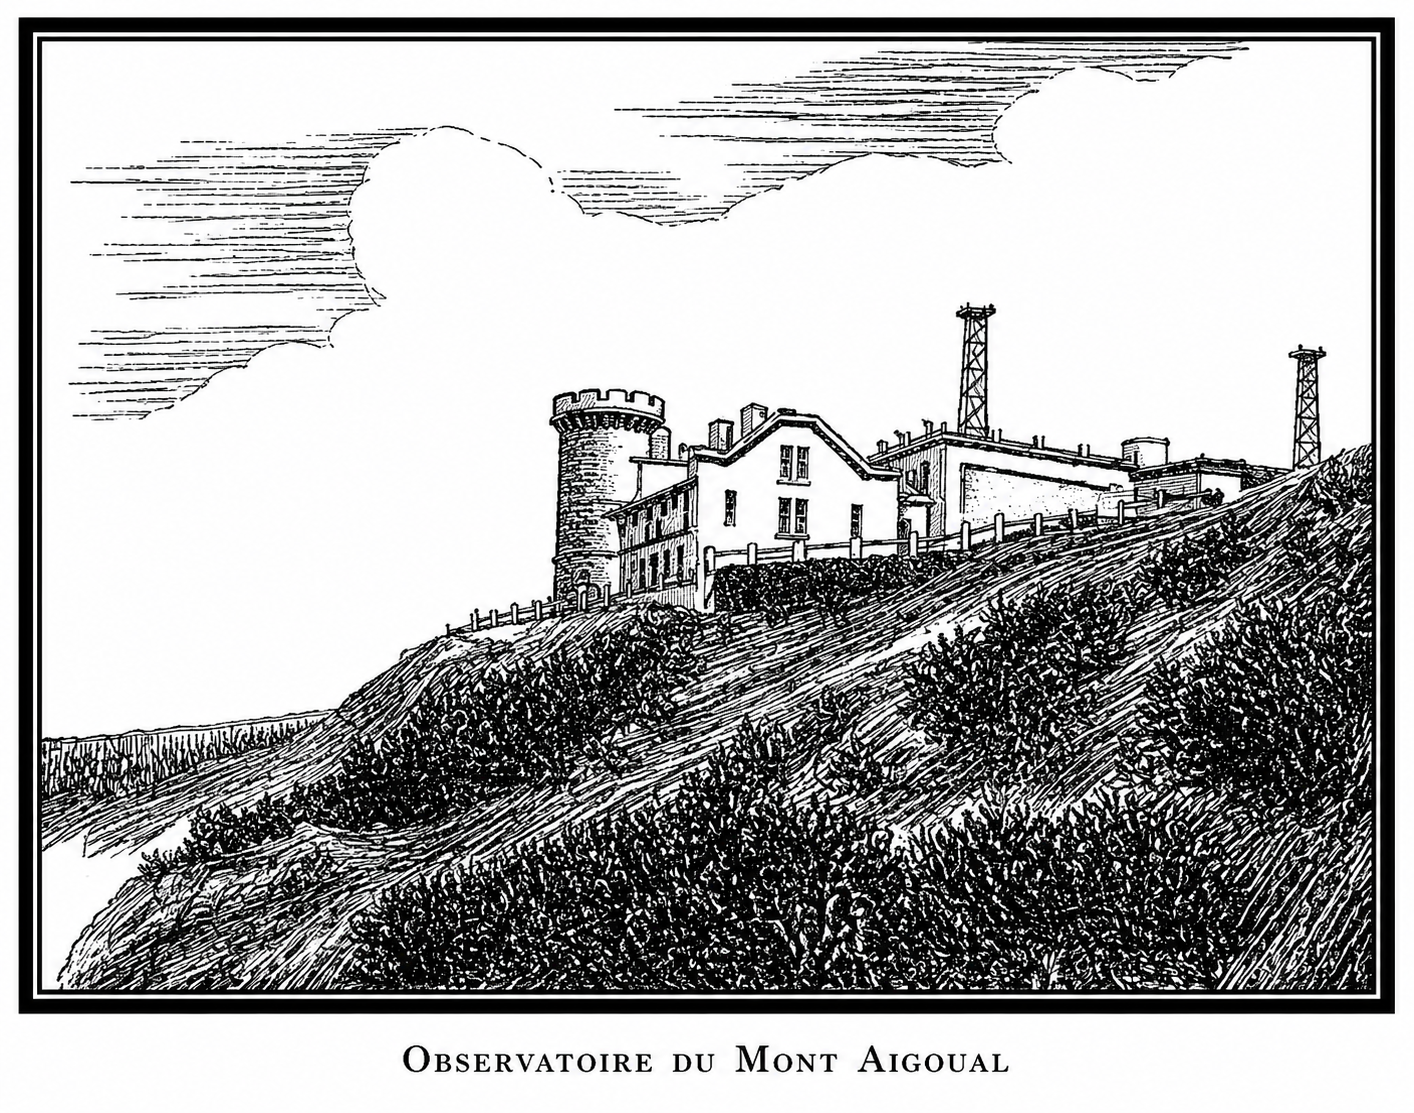
\includegraphics[width=\textwidth]{imgs/031.png}
\end{center}
